\section{搜索引擎}
\label{sec:search}

\subsection{简介}

随着越来越多的智能合约被开发者部署,用户面对海量的智能合约,搜索的需求也变得突出起来。智能合约仅仅是代码,并不包含任何功能描述,很难利用搜索引擎技术为智能合约建立索引。我们将用多种手段为智能合约建立合适的索引:
\begin{itemize}
	\item 爬取智能合约相关网页资料,为其和区块链智能合约建立映射关系;
	\item 鼓励开发者上传验证过的智能合约源代码,分析其代码功能和语义,为源代码建立索引,提供相似合约搜索;未提供源代码的智能合约,进行反编译得到其源代码;
	\item 为智能合约建立规范,任何符合此规范的智能合约,都能被检索并被用户搜索到,鼓励开发者在创建智能合约时,提供合约信息描述。
	\begin{lstlisting}[frame=single]
contract SearchableContract {
   string public language;
   string public author;
   string public name;
   string public title;
   string public description;
   string public tags;
}
	\end{lstlisting}
\end{itemize}

\subsection{搜索基础架构}

我们认为,搜索服务为了提供最佳的用户体验,中心化的架构更为适合。星云链开发组将实现一个搜索服务,实时检索所有智能合约,做多语言的分词,建立全文索引,最终提供一个友好的Web界面给用户使用。NR排序算法的公正性和每个节点的可验证性保证了中心化搜索服务的公正性,所有搜索后台代码都将开源给社区。第三方开发者也可据此创建独立的搜索服务。搜索服务架构如图\ref{fig:search-arch}所示。

\begin{figure}[h]
\centering
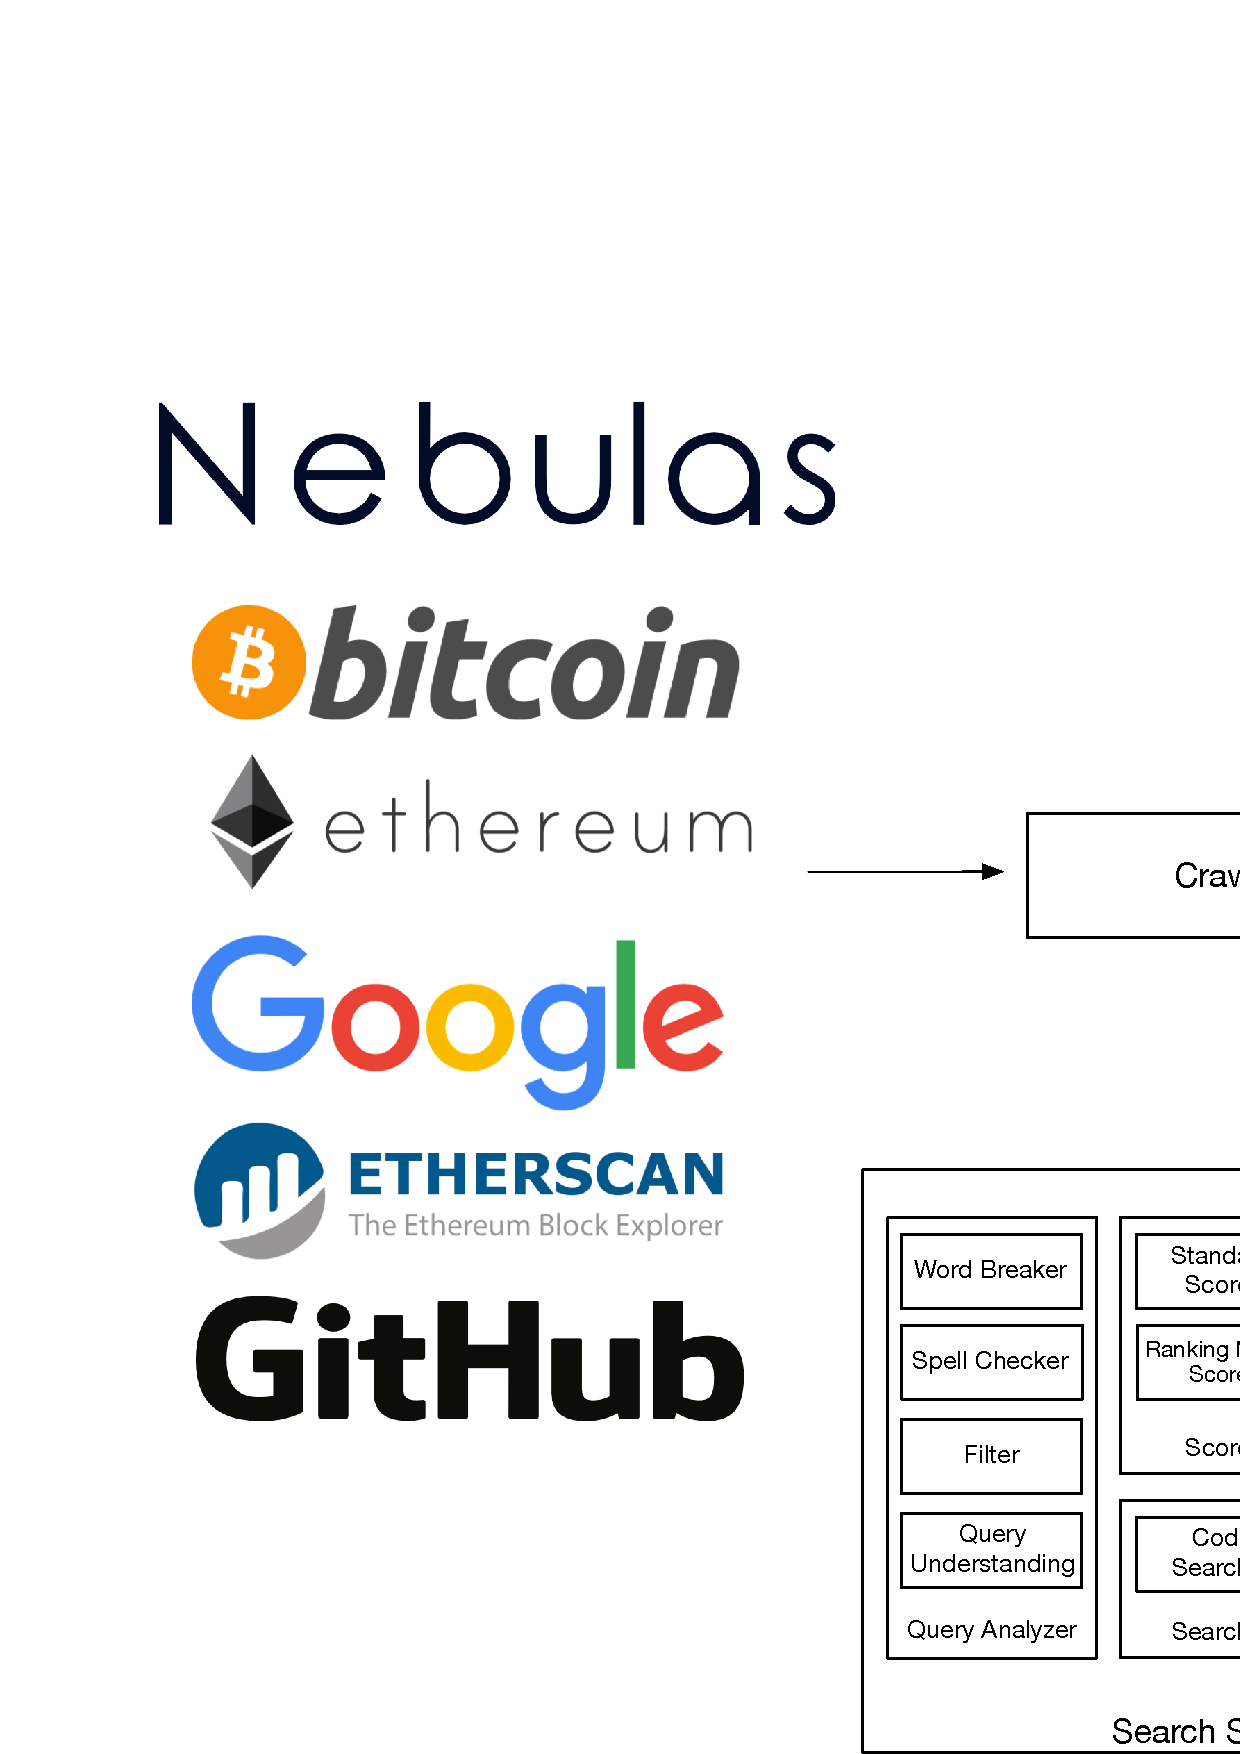
\includegraphics[width=16cm]{./figs/search-arch.pdf}
\caption{搜索服务架构}
\label{fig:search-arch}
\end{figure}

\begin{itemize}
	\item \textbf{Contract Extractor} 智能合约提取服务,从星云链中实时提取智能合约。
	\item \textbf{Crawler} 面向主题的智能合约网络爬虫,从公开网址爬取智能合约相关资料,包括介绍、Dapp用户评论、新闻资讯等。
	\item \textbf{Contract Analyzer} 智能合约分析器,包括合约反编译、源代码功能、语义分析,网页解析等。
	\item \textbf{Indexer} 从Contract Analyzer中建立合适的索引,支持全量和增量索引。
	\item \textbf{ElasticSearch Cluster} ES服务器集群。星云链团队考虑使用开源搜索引擎ElasticSearch作为其全文索引支持。
	\item \textbf{Rank Model Trainer} 排序模型训练。考虑到交易Graph,排序规则考虑了多个因素:匹配字段,文本相关度,合约的NR Rank值,合约的交易数量、频度和深度,与合约发生交易的用户NR Rank值,合约安全性等等。我们根据用户的实际使用情况,用机器学习算法(GBDT、人工神经网络都是候选)训练排序打分模型,根据用户的反馈不断优化。训练后的模型被搜索服务的Scorer使用。
	\item \textbf{Word Breaker} 多语言分词器,用作关键字搜索。
	\item \textbf{Scorer} 分为两个level:Level-1从ElasticSearch中召回候选结果集,目标是尽可能把潜在的候选结果,在ElasticSearch集群中通过快速有效的排序打分召回,Level-1召回的结果数量有限,控制在几千以内;Level-2使用Offline Rank Model,计算每个Level-1结果候选集的得分,重新排序,这个结果较为精确,可以直接给用户使用。
	\item \textbf{Searcher} 负责和ElasticSearch集群通信,以及对搜索结果包装返回给搜索前端。
\end{itemize}

\subsection{关键词搜索}
用户提供关键词,描述智能合约的标题、作者、功能等文本信息,在海量的智能合约中找到匹配的合约。对于文本搜索,目前有非常成熟的算法和技术,基于自然语言处理和倒排索引技术,我们可以在海量的智能合约索引库里高效的检索和排序。关键的技术如下:
\begin{enumerate}
	\item 面向主题的分布式爬虫技术
	\item 多语言分词技术:对于西文词汇,分词较为简单。对于中文分词,有多种算法可进行分词:正向最大匹配,逆向最大匹配,最短路径分词,统计分词等;
	\item 查询词纠错、语义理解
	\item 倒排索引,分布式搜索架构
	\item 超链排序算法:我们把区块链世界中用户之间的转账类比互联网世界的网页引用关系,提出NR排序算法。
\end{enumerate}


\subsection{相似代码搜索}
\todo{相似代码搜索算法待补充}

